\documentclass[11pt,a4paper]{article}
\usepackage[margin=2.5cm]{geometry}
\usepackage{booktabs}
\usepackage{graphicx}
\usepackage{xcolor}
\usepackage{hyperref}
\usepackage{enumitem}
\usepackage{titlesec}
\usepackage{fancyhdr}
\usepackage{microtype}
\usepackage{parskip}
\usepackage{fontspec}
\usepackage{polyglossia}
\usepackage{amsmath}
\usepackage{amssymb}

\setmainlanguage{english}
\setotherlanguage{hebrew}
\newfontfamily\hebrewfont{DejaVu Sans}[Script=Hebrew]

\hypersetup{colorlinks=true, linkcolor=blue, urlcolor=blue}

\pagestyle{fancy}
\fancyhf{}
\rhead{Knesset Protocol Journal Project}
\lhead{Step 3 --- Dense De-Anisotropization}
\rfoot{Page \thepage}
\lfoot{Tomer Morad, Or Israeli, Yoel Marko --- June 2026}

\titleformat{\section}{\large\bfseries}{\thesection.}{0.6em}{}[\titlerule]
\titleformat{\subsection}{\normalsize\bfseries}{\thesubsection}{0.6em}{}

\begin{document}

\begin{center}
  {\LARGE \textbf{De-Anisotropizing Dense Embeddings with ABTT}}\\[0.3em]
  {\large Step 3 --- Removing the parliamentary-register bias from sentence vectors}\\[0.6em]
  {\normalsize Tomer Morad \quad Or Israeli \quad Yoel Marko}\\
  {\normalsize June 2026}
\end{center}

\vspace{0.5em}

% ----------------------------------------------------------------------
\section{Objective}

Step 2 revealed that off-the-shelf dense embeddings of Knesset committee text are
\textbf{severely anisotropic}: the cosine similarity between \emph{any} two spans is
$\approx$0.95 for \texttt{e5} and $\approx$0.98 for AlephBERT regardless of their gold topic,
leaving a discrimination gap of only 0.007--0.018.  This collapses clustering performance
well below TF-IDF (ARI$_\text{km}$ = 0.377 for TF-IDF vs.\ 0.322 for \texttt{e5}).

The hypothesis is that this isotropy is driven by a small number of directions shared across
all committee discussions --- the voice of a single Knesset committee's procedural Hebrew
(standard openings, motions, voting formulae).  Projecting out these directions should
widen the same-vs-different-topic margin and restore topic discriminability.

% ----------------------------------------------------------------------
\section{Method: All-But-The-Top (ABTT)}

We apply the All-But-The-Top postprocessing introduced by Mu \& Viswanath (ICLR 2018)
(originally for static word vectors; applies equally to sentence embeddings):

\begin{enumerate}[noitemsep]
  \item \textbf{Center.} Subtract the mean of all 198 span vectors: $\hat{X} = X - \bar{x}$.
  \item \textbf{Identify dominant directions.} Compute the economy SVD of $\hat{X}$;
        let $V \in \mathbb{R}^{k \times d}$ be the top-$k$ right singular vectors.
  \item \textbf{Project out.} Remove the subspace spanned by $V$:
        $\tilde{X} = \hat{X} - (\hat{X} V^\top) V$.
  \item \textbf{Re-normalize.} L2-normalize each row of $\tilde{X}$.
\end{enumerate}

We sweep $k \in \{0, 1, 2, 3, 5, 7, 10, 15, 20, 30, 50\}$ for each model
(\texttt{e5}-large-1024d, \texttt{mpnet}-768d, \texttt{alephbert}-768d).
$k=0$ is the normalized baseline (same as Step 2, modulo centering).
The PCA is fit on all 198 spans; evaluation is on the 105-span recurring subset.

% ----------------------------------------------------------------------
\section{Results}

\subsection{Quantitative summary}

\begin{center}
\begin{tabular}{lcccccc}
\toprule
\textbf{Configuration} & \textbf{Best $k$} & \textbf{ARI$_\text{km}$} & \textbf{ARI$_\text{agg}$} & \textbf{AUC} & \textbf{sim gap} \\
\midrule
\textbf{TF-IDF (baseline)} & --- & 0.377 & 0.249 & 0.741 & 0.069 \\
\midrule
\texttt{e5}, $k=0$ (raw) & --- & 0.322 & 0.136 & 0.744 & 0.018 \\
\texttt{e5}, $k=1$        & 1   & 0.363 & \textbf{0.540} & \textbf{0.899} & 0.343 \\
\texttt{e5}, $k=3$        & \textbf{3}   & 0.375 & 0.442 & 0.861 & 0.259 \\
\midrule
\texttt{mpnet}, $k=0$ (raw) & --- & 0.169 & 0.221 & 0.740 & 0.066 \\
\texttt{mpnet}, $k=10$ & 10 & 0.314 & 0.309 & 0.707 & 0.173 \\
\midrule
\texttt{alephbert}, $k=0$ (raw) & --- & 0.224 & 0.113 & 0.632 & 0.007 \\
\textbf{\texttt{alephbert}, $k=2$} & \textbf{2} & \textbf{0.391} & 0.513 & 0.887 & 0.344 \\
\bottomrule
\end{tabular}
\end{center}

\noindent\textbf{AlephBERT $k=2$ beats TF-IDF} on KMeans ARI (0.391 vs.\ 0.377) --- the first
dense configuration to do so.  \texttt{e5} $k=1$ achieves the highest agglomerative ARI (0.540,
a 2$\times$ improvement over TF-IDF's 0.249) and the highest AUC (0.899).

\subsection{The anisotropy was concentrated in 1--2 principal components}

The similarity gap --- the key diagnostic from Step 2 --- improves dramatically with even
a single component removed:

\begin{center}
\begin{tabular}{lcccc}
\toprule
\textbf{Model} & \textbf{gap, $k=0$} & \textbf{gap, $k=1$} & \textbf{gap, $k=2$} & \textbf{gap, $k=3$} \\
\midrule
\texttt{e5}        & 0.018 & 0.343 & 0.264 & 0.259 \\
\texttt{alephbert} & 0.007 & 0.333 & \textbf{0.344} & 0.252 \\
\midrule
TF-IDF & \multicolumn{4}{c}{0.069 (constant)} \\
\bottomrule
\end{tabular}
\end{center}

\noindent The first PC alone accounts for the bulk of the improvement.  This is consistent
with the hypothesis: a \emph{single} ``committee register'' direction dominates all 198 span
vectors, and removing it unlocks the topic-discriminative signal already latent in the encoder.

\subsection{Over-removal degrades performance}

Beyond $k\approx5$, performance degrades monotonically as topic-discriminative directions
are also projected out.  The sweet spot of $k=1$--$3$ is consistent across all three models.

\begin{center}
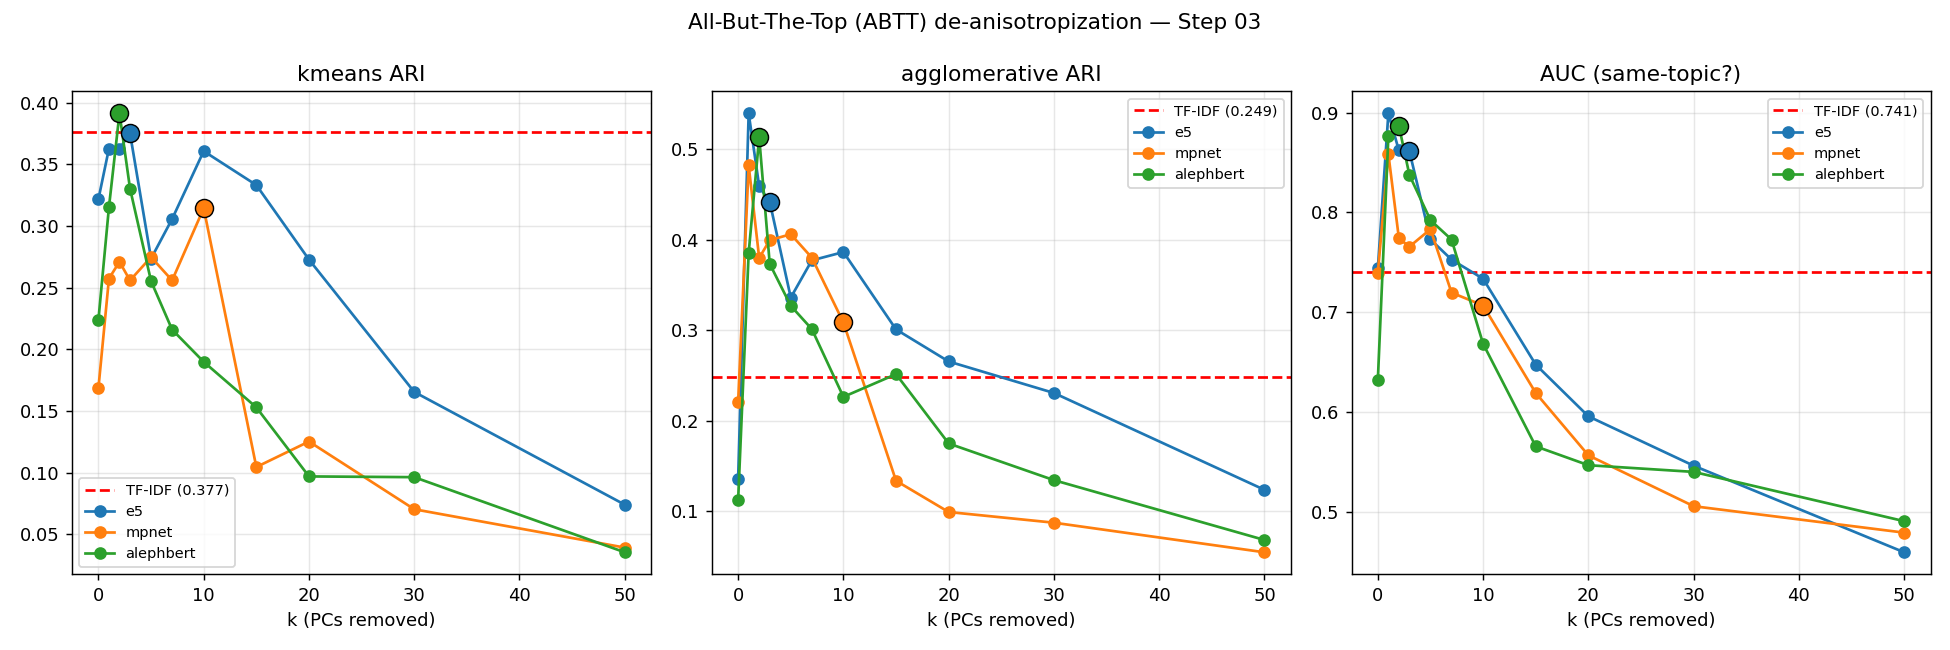
\includegraphics[width=\textwidth]{../outputs/abtt_curves.png}
\end{center}
\noindent KMeans ARI, Agglomerative ARI, and same-topic AUC as a function of $k$.
The red dashed line is the TF-IDF baseline.  Filled circles mark the best $k$ per model.

% ----------------------------------------------------------------------
\section{Takeaways}

\begin{itemize}[noitemsep]
  \item The anisotropy in Knesset committee embeddings is a \textbf{low-rank phenomenon}:
        $k=2$ PCs suffice to encode almost all of the domain-register bias.
  \item \textbf{ABTT with $k=2$ enables AlephBERT to surpass TF-IDF} --- a result
        achievable in milliseconds of CPU postprocessing with no additional training.
  \item \textbf{\texttt{e5} $k=1$ is the AUC champion} (0.899 vs.\ 0.741 for TF-IDF),
        making it the natural choice for the similarity-threshold Task-2 baseline.
  \item The technique is \emph{architecture-agnostic}: it works on any encoder whose
        output is dominated by a shared register subspace.
\end{itemize}

% ----------------------------------------------------------------------
\section{Future Directions}

\begin{enumerate}[leftmargin=1.4em]
  \item \textbf{Hybrid TF-IDF + ABTT score fusion.}  TF-IDF contributes lexical precision
        (bill IDs, entity names) while ABTT-corrected dense contributes paraphrase recall.
        A weighted combination $\alpha \cdot S_\text{tfidf} + (1-\alpha) \cdot S_\text{dense}$
        should improve over either component alone.  (Implemented in Step 4.)
  \item \textbf{Finer sweep near $k=1$--$2$.}  Fractional whitening (scale rather than
        zero-out singular directions) may give smoother trade-offs.
  \item \textbf{Centroid-based representative in streaming.}  Rather than using the first
        span as a journal-entry representative, maintain an ABTT-corrected centroid that
        updates as the entry accumulates spans.
\end{enumerate}

\vspace{1.5em}
\hrule
\vspace{0.4em}
{\small
\textbf{Artifacts (this step):}
\texttt{outputs/abtt\_results.json},
\texttt{outputs/abtt\_curves.png},
\texttt{outputs/best\_embeddings/\{model\}\_abtt\_k\{k\}.npy}.\\
\textbf{Code:} \texttt{code/deanisotrize\_eval.py}.
}

\end{document}
